\documentclass{article}
\usepackage[utf8]{inputenc}
\usepackage{amsmath}
\usepackage{amssymb}
\usepackage{amsthm}
\usepackage[colorlinks=true]{hyperref}
\usepackage{parskip}
\usepackage{tikz}
\usetikzlibrary{arrows,automata}

\title{INF2080\\Oblig 1}
\date{\textbf{Deadline:} February 19, 2016}

\setcounter{secnumdepth}{0}

\begin{document}

\maketitle

\section{Hand-in and deadline}
Hand in a single PDF file in \href{https://devilry.ifi.uio.no/}{Devilry}. Deadline is \textbf{February 19, at 23:59}.

We recommend \LaTeX{}, but all major text editors allows exporting to PDF. You can get help with \LaTeX{} at the group sessions. You can also download the \LaTeX{} source (\texttt{.tex}) for this assignment at the assignments page.

\section{Problem 1: Regular languages}
Let $A$ and $B$ be regular languages defined by DFAs $\mathcal A$ and $\mathcal B$. Let $n_\mathcal A$ and $n_\mathcal B$ be the number of states in $\mathcal A$ and $\mathcal B$.

\subsection{Problem 1a}
What are the highest number of states you would need in \textbf{DFAs} for the languages $A\cap B$ and $A^*$?

\subsection{Problem 1b}
What are the highest number of states you would need in \textbf{NFAs} for the languages $A\cap B$, $AB$ and $A^*$?

\subsection{Problem 1c}
Create a regular expression defining the same language as the DFA

\begin{center}
    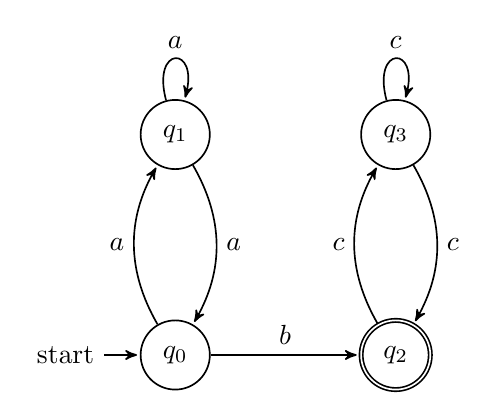
\begin{tikzpicture}[->,>=stealth',shorten >=1pt,auto,node distance=2.8cm,
                        semithick]

        \node[initial,state] (q0) {$q_0$};
        \node[state] (q1) [above of=q0] {$q_1$};
        \node[state,accepting] (q2) [right of=q0] {$q_2$};
        \node[state] (q3) [above of=q2] {$q_3$};

        \path (q0) edge [bend left] node {$a$} (q1)
                    edge node {$b$} (q2)
                (q1) edge [loop above] node {$a$} (q1)
                    edge [bend left] node {$a$} (q0)
                (q2) edge [bend left] node {$c$} (q3)
                (q3) edge [loop above] node {$c$} (q3)
                    edge [bend left] node {$c$} (q2);
    \end{tikzpicture}
\end{center}

\subsection{Problem 1d}
Create a DFA for the language
\begin{align*}
    \{w\mid \text{$w$ contains equally many occurences of the substrings 01 and 10}\}.
\end{align*}

\section{Problem 2: all-NFAs}
An all-NFA is defined in Sipser, problem 1.43 as a 5-tuple $(Q,\Sigma,\delta,q_0,F)$ that accepts $x\in\Sigma^*$ if \emph{every} possible state that $M$ could reach after reading input $x$ is in $F$ (as opposed to \emph{at least one}).

If any brach in an all-NFA computation reaches an inplicit or explicit sink state, the input is not accepted.

Show how any all-NFA can be converted to a DFA.

\section{Problem 3: Non-regular languages}
The DFA
\begin{center}
    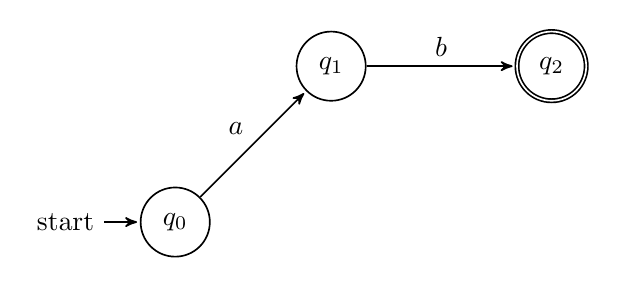
\begin{tikzpicture}[->,>=stealth',shorten >=1pt,auto,node distance=2.8cm,
                        semithick]

        \node[initial,state] (q0) {$q_0$};
        \node[state] (q1) [above right of=q0] {$q_1$};
        \node[state,accepting] (q2) [right of=q1] {$q_2$};

        \path (q0) edge node {$a$} (q1)
                (q1) edge node {$b$} (q2);
    \end{tikzpicture}
\end{center}
defines the language $\{ab\}$. The DFA
\begin{center}
    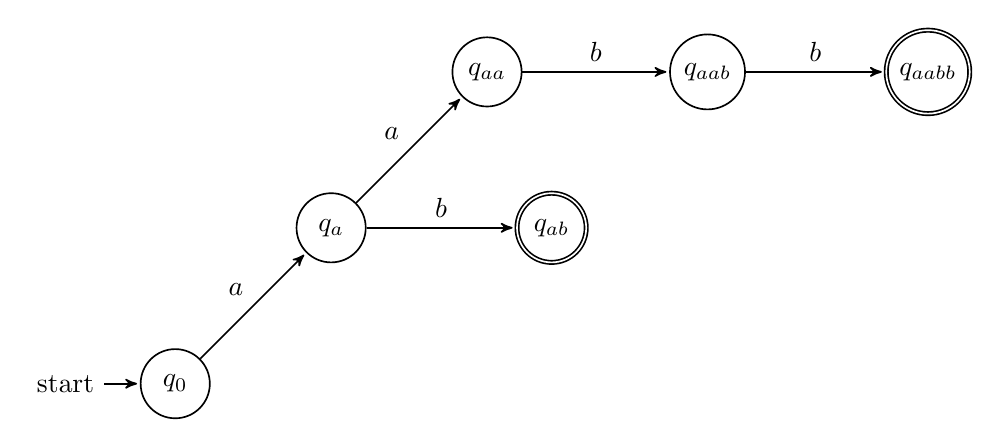
\begin{tikzpicture}[->,>=stealth',shorten >=1pt,auto,node distance=2.8cm,
                        semithick]

        \node[initial,state] (q0) {$q_0$};
        \node[state] (qa) [above right of=q0] {$q_{a}$};
        \node[state,accepting] (qab) [right of=qa] {$q_{ab}$};
        \node[state] (qaa) [above right of=qa] {$q_{aa}$};
        \node[state] (qaab) [right of=qaa] {$q_{aab}$};
        \node[state,accepting] (qaabb) [right of=qaab] {$q_{aabb}$};

        \path (q0) edge node {$a$} (qa)
                (qa) edge node {$b$} (qab)
                    edge node {$a$} (qaa)
                (qaa) edge node {$b$} (qaab)
                (qaab) edge node {$b$} (qaabb);
    \end{tikzpicture}
\end{center}
defines the language $\{ab,aabb\}$.

\subsection{Problem 3a}
Create a DFA that defines the language $\{ab,aabb,aaabbb\}$.

\subsection{Problem 3b}
Create a deterministic \emph{infinite} automaton that defines the language
\begin{align*}
    \{a^n b^n\mid n\in\mathbb N\}.
\end{align*}

\subsection{Problem 3c}
Using the pumping lemma, give a detailed proof that $\{a^n b^n\mid n\in\mathbb N\}$ is not a regular language; that is, no deterministic \emph{finite} automaton may define it.

\subsection{Problem 3d}
Show that $\{a^n b^n\mid n\in\mathbb N\}$ is a context free language.



\end{document}